\documentclass[a4paper,14pt,oneside,openany]{memoir}
  
%%% Задаем поля, отступы и межстрочный интервал %%%

\usepackage[left=30mm, right=15mm, top=20mm, bottom=20mm]{geometry} % Пакет geometry с аргументами для определения полей

% Please add the following required packages to your document preamble:
\usepackage{graphicx}
\usepackage{lscape}
\usepackage{longtable}
\usepackage{enumitem}
\setlist[enumerate,1]{label=\arabic*)}

\pagestyle{plain} % Убираем стандарные для данного класса верхние колонтитулы с заголовком текущей главы, оставляем только номер страницы снизу по центру
\parindent=1.25cm % Абзацный отступ 1.25 см, приблизительно равно пяти знакам, как по ГОСТ
\usepackage{indentfirst} % Добавляем отступ к первому абзацу
%\linespread{1.3} % Межстрочный интервал (наиболее близко к вордовскому полуторному) - тут вместо этого используется команда OnehalfSpacing*

%%% Задаем языковые параметры и шрифт %%%

\usepackage[english, russian]{babel}                % Настройки для русского языка как основного в тексте
\babelfont{rm}{Times New Roman}                     % TMR в качестве базового roman-щрифта

%%% Задаем стиль заголовков и подзаголовков в тексте %%%

\setsecnumdepth{subsection} % Номера разделов считать до третьего уровня включительно, т.е. нумеруются только главы, секции, подсекции
\renewcommand*{\chapterheadstart}{} % Переопределяем команду, задающую отступ над заголовком, чтобы отступа не было
\renewcommand*{\printchaptername}{} % Переопределяем команду, печатающую слово "Глава", чтобы оно не печалось
%\renewcommand*{\printchapternum}{} % То же самое для номера главы - тут не надо, номер главы оставляем
\renewcommand*{\chapnumfont}{\normalfont\bfseries} % Меняем стиль шрифта для номера главы: нормальный размер, полужирный
\renewcommand*{\afterchapternum}{\hspace{1em}} % Меняем разделитель между номером главы и названием
\renewcommand*{\printchaptertitle}{\normalfont\bfseries\centering\MakeUppercase} % Меняем стиль написания для заголовка главы: нормальный размер, полужирный, центрированный, заглавными буквами
\setbeforesecskip{20pt} % Задаем отступ перед заголовком секции
\setaftersecskip{20pt} % Ставим такой же отступ после заголовка секции
\setsecheadstyle{\raggedright\normalfont\bfseries} % Меняем стиль написания для заголовка секции: выравнивание по правому краю без переносов, нормальный размер, полужирный
\setbeforesubsecskip{20pt} % Задаем отступ перед заголовком подсекции
\setaftersubsecskip{20pt} % Ставим такой же отступ после заголовка подсекции
\setsubsecheadstyle{\raggedright\normalfont\bfseries}  % Меняем стиль написания для заголовка подсекции: выравнивание по правому краю без переносов, нормальный размер, полужирный

%%% Задаем параметры оглавления %%%

\addto\captionsrussian{\renewcommand\contentsname{Содержание}} % Меняем слово "Оглавление" на "Содержание"
\setrmarg{2.55em plus1fil} % Запрещаем переносы слов в оглавлении
%\setlength{\cftbeforechapterskip}{0pt} % Эта команда убирает интервал между заголовками глав - тут не надо, так красивее смотрится
\renewcommand{\aftertoctitle}{\afterchaptertitle \vspace{-\cftbeforechapterskip}} % Делаем отступ между словом "Содержание" и первой строкой таким же, как у заголовков глав
%\renewcommand*{\chapternumberline}[1]{} % Делаем так, чтобы номер главы не печатался - тут не надо
\renewcommand*{\cftchapternumwidth}{1.5em} % Ставим подходящий по размеру разделитель между номером главы и самим заголовком
\renewcommand*{\cftchapterfont}{\normalfont\MakeUppercase} % Названия глав обычным шрифтом заглавными буквами
\renewcommand*{\cftchapterpagefont}{\normalfont} % Номера страниц обычным шрифтом
\renewcommand*{\cftchapterdotsep}{\cftdotsep} % Делаем точки до номера страницы после названий глав
\renewcommand*{\cftdotsep}{1} % Задаем расстояние между точками
\renewcommand*{\cftchapterleader}{\cftdotfill{\cftchapterdotsep}} % Делаем точки стандартной формы (по умолчанию они "жирные")
\maxtocdepth{subsection} % В оглавление попадают только разделы первыхтрех уровней: главы, секции и подсекции

%%% Выравнивание и переносы %%%

%% http://tex.stackexchange.com/questions/241343/what-is-the-meaning-of-fussy-sloppy-emergencystretch-tolerance-hbadness
%% http://www.latex-community.org/forum/viewtopic.php?p=70342#p70342
\tolerance 1414
\hbadness 1414
\emergencystretch 1.5em                             % В случае проблем регулировать в первую очередь
\hfuzz 0.3pt
\vfuzz \hfuzz
%\dbottom
%\sloppy                                            % Избавляемся от переполнений
\clubpenalty=10000                                  % Запрещаем разрыв страницы после первой строки абзаца
\widowpenalty=10000                                 % Запрещаем разрыв страницы после последней строки абзаца
\brokenpenalty=4991                                 % Ограничение на разрыв страницы, если строка заканчивается переносом

%%% Объясняем компилятору, какие буквы русского алфавита можно использовать в перечислениях (подрисунках и нумерованных списках) %%%
%%% По ГОСТ нельзя использовать буквы ё, з, й, о, ч, ь, ы, ъ %%%
%%% Здесь также переопределены заглавные буквы, хотя в принципе они в документе не используются %%%

\makeatletter
    \def\russian@Alph#1{\ifcase#1\or
       А\or Б\or В\or Г\or Д\or Е\or Ж\or
       И\or К\or Л\or М\or Н\or
       П\or Р\or С\or Т\or У\or Ф\or Х\or
       Ц\or Ш\or Щ\or Э\or Ю\or Я\else\xpg@ill@value{#1}{russian@Alph}\fi}
    \def\russian@alph#1{\ifcase#1\or
       а\or б\or в\or г\or д\or е\or ж\or
       и\or к\or л\or м\or н\or
       п\or р\or с\or т\or у\or ф\or х\or
       ц\or ш\or щ\or э\or ю\or я\else\xpg@ill@value{#1}{russian@alph}\fi}
\makeatother

%%% Задаем параметры оформления рисунков и таблиц %%%

\usepackage{graphicx, caption, subcaption} % Подгружаем пакеты для работы с графикой и настройки подписей
\graphicspath{{images/}} % Определяем папку с рисунками
\captionsetup[figure]{font=small, width=\textwidth, name=Рисунок, justification=centering} % Задаем параметры подписей к рисункам: маленький шрифт (в данном случае 12pt), ширина равна ширине текста, полнотекстовая надпись "Рисунок", выравнивание по центру
\captionsetup[subfigure]{font=small} % Индексы подрисунков а), б) и так далее тоже шрифтом 12pt (по умолчанию делает еще меньше)
\captionsetup[table]{singlelinecheck=false,font=small,width=\textwidth,justification=justified} % Задаем параметры подписей к таблицам: запрещаем переносы, маленький шрифт (в данном случае 12pt), ширина равна ширине текста, выравнивание по ширине
\captiondelim{ --- } % Разделителем между номером рисунка/таблицы и текстом в подписи является длинное тире
\setkeys{Gin}{width=\textwidth} % По умолчанию размер всех добавляемых рисунков будет подгоняться под ширину текста
\renewcommand{\thesubfigure}{\asbuk{subfigure}} % Нумерация подрисунков строчными буквами кириллицы
%\setlength{\abovecaptionskip}{0pt} % Отбивка над подписью - тут не меняем
%\setlength{\belowcaptionskip}{0pt} % Отбивка под подписью - тут не меняем
\usepackage[section]{placeins} % Объекты типа float (рисунки/таблицы) не вылезают за границы секциии, в которой они объявлены

%%% Задаем параметры ссылок и гиперссылок %%% 

\usepackage{hyperref}                               % Подгружаем нужный пакет
\hypersetup{
    colorlinks=true,                                % Все ссылки и гиперссылки цветные
    linktoc=all,                                    % В оглавлении ссылки подключатся для всех отображаемых уровней
    linktocpage=true,                               % Ссылка - только номер страницы, а не весь заголовок (так выглядит аккуратнее)
    linkcolor=black,                                  % Цвет ссылок и гиперссылок - красный
    citecolor=black                                   % Цвет цитировний - красный
}

%%% Настраиваем отображение списков %%%

\usepackage{enumitem}                               % Подгружаем пакет для гибкой настройки списков
\renewcommand*{\labelitemi}{\normalfont{--}}        % В ненумерованных списках для пунктов используем короткое тире
\makeatletter
    \AddEnumerateCounter{\asbuk}{\russian@alph}     % Объясняем пакету enumitem, как использовать asbuk
\makeatother
\renewcommand{\labelenumii}{\asbuk{enumii})}        % Кириллица для второго уровня нумерации
\renewcommand{\labelenumiii}{\arabic{enumiii})}     % Арабские цифры для третьего уровня нумерации
\setlist{noitemsep, leftmargin=*}                   % Убираем интервалы между пунками одного уровня в списке
\setlist[1]{labelindent=\parindent}                 % Отступ у пунктов списка равен абзацному отступу
\setlist[2]{leftmargin=\parindent}                  % Плюс еще один такой же отступ для следующего уровня
\setlist[3]{leftmargin=\parindent}                  % И еще один для третьего уровня

%%% Счетчики для нумерации объектов %%%

\counterwithout{figure}{chapter}                    % Сквозная нумерация рисунков по документу
\counterwithout{equation}{chapter}                  % Сквозная нумерация математических выражений по документу
\counterwithout{table}{chapter}                     % Сквозная нумерация таблиц по документу

%%% Реализация библиографии пакетами biblatex и biblatex-gost с использованием движка biber %%%

\usepackage{csquotes} % Пакет для оформления сложных блоков цитирования (biblatex рекомендует его подключать)
\usepackage[%
backend=biber,                                      % Движок
bibencoding=utf8,                                   % Кодировка bib-файла
sorting=none,                                       % Настройка сортировки списка литературы
style=gost-numeric,                                 % Стиль цитирования и библиографии по ГОСТ
language=auto,                                      % Язык для каждой библиографической записи задается отдельно
autolang=other,                                     % Поддержка многоязычной библиографии
sortcites=true,                                     % Если в квадратных скобках несколько ссылок, то отображаться будут отсортированно
movenames=false,                                    % Не перемещать имена, они всегда в начале библиографической записи
maxnames=5,                                         % Максимальное отображаемое число авторов
minnames=3,                                         % До скольки сокращать число авторов, если их больше максимума
doi=false,                                          % Не отображать ссылки на DOI
isbn=false,                                         % Не показывать ISBN, ISSN, ISRN
]{biblatex}[2016/09/17]
\DeclareDelimFormat{bibinitdelim}{}                 % Убираем пробел между инициалами (Иванов И.И. вместо Иванов И. И.)
\addbibresource{biba.bib}                           % Определяем файл с библиографией

%%% Скрипт, который автоматически подбирает язык (и, следовательно, формат) для каждой библиографической записи %%%
%%% Если в названии работы есть кириллица - меняем значение поля langid на russian %%%
%%% Все оставшиеся пустые места в поле langid заменяем на english %%%

\DeclareSourcemap{
  \maps[datatype=bibtex]{
    \map{
        \step[fieldsource=title, match=\regexp{^\P{Cyrillic}*\p{Cyrillic}.*}, final]
        \step[fieldset=langid, fieldvalue={russian}]
    }
    \map{
        \step[fieldset=langid, fieldvalue={english}]
    }
  }
}

%%% Прочие пакеты для расширения функционала %%%

\usepackage{longtable,ltcaption}                    % Длинные таблицы
\usepackage{multirow,makecell}                      % Улучшенное форматирование таблиц
\usepackage{booktabs}                               % Еще один пакет для красивых таблиц
\usepackage{soulutf8}                               % Поддержка переносоустойчивых подчёркиваний и зачёркиваний
\usepackage{icomma}                                 % Запятая в десятичных дробях
\usepackage{hyphenat}                               % Для красивых переносов
\usepackage{textcomp}                               % Поддержка "сложных" печатных символов типа значков иены, копирайта и т.д.
\usepackage[version=4]{mhchem}                      % Красивые химические уравнения
\usepackage{amsmath}                                % Усовершенствование отображения математических выражений 
  
%%% Вставляем по очереди все содержательные части документа %%%


\usepackage{setspace}

\begin{document}
\OnehalfSpacing* % Задаем полуторный интервал текста (в титульнике одинарный, поэтому команда стоит после него)

\pagenumbering{gobble} % Страницы без нумерации
\chapter*{Реферат}
\label{ch:referat}
\linespread{1.5}

Выпускная квалификационная работа бакалавра 48 с., 12 рис., 5 табл., 58 источн.

\noindent

 МОДЕЛЬ ДЛЯ ПРОГНОЗИРОВАНИЯ ЗАБОЛЕВАЕМОСТИ ВИЧ, ЭПИДЕМИЯ ВИЧ/СПИД, ИСПОЛЬЗОВАНИЕ СОЦИАЛЬНО-ДЕМОГРАФИЧЕСКИХ ПРЕДИКТОРОВ, НЕЙРОННЫЕ СЕТИ В СОЧЕТАНИИ С КЛАССИЧЕСКИМИ СТАТИСТИЧЕСКИМИ МЕТОДАМИ, ПОЛУЧЕНИЕ ПРОГНОЗА

Объект исследования - эпидемия ВИЧ/СПИД.

Предмет исследования - методы прогнозирования заболеваемости с использованием нейронных сетей.

Методы исследования: анализ, синтез, формализация, моделирование, сравнение, измерение.

Результат работы: сформулирован вывод об эффективности применения нейронных сетей для задач прогнозирования ВИЧ-инфекции в субъектах Российской Федерации, разработана нейросетевая модель для прогнозоирования с учетом дополнительных социально-демографических факторов, получено финальное предсказание с применением наиболее актуальных данных.


\endinput                                     % Реферат
\newpage

\tableofcontents*                                   % Автособираемое оглавление
\clearpage  % Начинаем считать номера страниц со шестой
\pagenumbering{arabic}
\setcounter{page}{6}

\chapter*{Введение}
\addcontentsline{toc}{chapter}{Введение}
\label{ch:intro}
\linespread{1.5}
    В современном мире проблема ВИЧ/СПИД остается одной из наиболее актуальных и серьезных в области здравоохранения по всему миру, в том числе в Российской Федерации. Обратимся к наиболее актуальным данным Федерального научно-методического центра по борьбе со СПИДом (Роспотребнадзора) \cite{Справка_по_ВИЧ-инфекции_в_России_Роспотребнадзор_2022} и приведем несколько ключевых положений статистики за 2022 год: 
    
\begin{enumerate}
    \item  На момент 31 декабря 2022 г. в стране проживало 1 168 076 россиян с лабораторно подтвержденным диагнозом ВИЧ-инфекции, исключая 461 879 больных, умерших за весь период наблюдения с 1987 года.
    
    \item Всего зарегистрировано 63 150 новых случаев болезни, вызванных вирусом иммунодефицита человека. Показатель заболеваемости при этом равен 43,29 на 100 тыс. населения, что на 3,8 \% больше, чем в 2021 и 2020 годах.
    
    \item На диспансерном учете состояло 835 154 больных, то есть 69,5 \% от числа россиян, живущих с диагностированной ВИЧ-инфекцией. Получали антиретровирусную терапию в 711 412 пациентов, что составляет 85,2 \% от числа состоявших на диспансерном наблюдении и 59,2 \% от общего числа живущих с диагнозом ВИЧ-инфекция.

    \item В 2022 г. было сообщено о смерти 34 410 инфицированных ВИЧ россиян, что больше чем в 2021 г. (на 0,9 \%), в 2020 г. (на 6,8 \%) и в 2019 г. (на 2,4 \%). Поскольку ВИЧ-инфекция является неизлечимым заболеванием, а число новых случаев ВИЧ-инфекции превышает число умерших, общее число россиян, живущих с ВИЧ, продолжает расти.
    
    \item По словам исследователей, <<Эпидемия ВИЧ-инфекции продолжает развиваться, и кроме увеличения охвата ВИЧ-позитивного 
    населения лечением, необходимо развитие комплекса программ по предотвращению заражения ВИЧ>>.    
    
\end{enumerate}


    Помимо высоких показателей смертности и заболеваемости, ВИЧ-инфекция также характеризуется социальной значимостью, связанной с высокой степенью стигматизации и дискриминации носителей инфекции. Некоторые люди до сих пор считают ВИЧ-инфекцию <<заслуженной>> болезнью, которая угрожает только наркоманам и людям, ведущими беспорядочную половую жизнь. Корнями эти предубеждения уходят во времена возникновения первых случаев ВИЧ в СССР, когда подобные мнения были распространены в СМИ и поддерживались местными органами власти. Так, В 1986 г. министр здравоохранения РСФСР Николай Трубилин в программе «Время» заявил:

    «В Америке СПИД бушует с 1981 года, это западная болезнь. У нас нет базы для распространения этой инфекции, так как в России нет наркомании и проституции»\cite{ВИЧ_СССР_цитата_Министра}.

    Чтобы проиллюстрировать отношение к ВИЧ в современной России, обратимся к результатам социальных опросов, проведенных в 2015 году среди 256 студентов-первокурсников в рамках научно-исследовательской работы <<ВИЧ-инфекция как социальная проблема>> \cite{Вич_социальная_проблема2015}:
    
\begin{enumerate}

    \item  38,3 \% опрошенных считают необходимым изолировать себя/своих детей от общения с ВИЧ-инфицированными людьми (избегать общения/перевести ребенка в другой класс и т.д.), 14,4 \% затрудняются ответить на данный вопрос.
    \item  9 \% опрошенных считают, что диагноз ВИЧ необходимо скрывать от друзей и знакомых, 55 \% затрудняются ответить на данный вопрос.
    \item  49 \% опрошенных считают ВИЧ-инфицированных людей асоциальными в той или иной степени.
    \item Всего 11,3 \% опрошенных узнали о ВИЧ-инфекции из уст родителей, остальные получили информацию из СМИ (66,4 \%), интернета (5,9 \%), со слов сверстников (4,3 \%) и из прочих источников.
\end{enumerate}

    Точной статистики о числе случаев дискриминации ВИЧ-инфицированных в России нет, однако, согласно информации из разных источников \cite{Современная_российская_проблематика,spid_center_2862_discrimination, spid_center_1458_discrimination}, такие люди часто сталкиваются с незаконным (ч.1 ст. 137 УК РФ) разглашением их диагноза третьими лицами, в том числе друзьями и медицинскими сотрудниками, трудностями в работе и учебе, связанными с социальной депривацией, отказом от предоставления медицинских услуг со стороны врачей, недостаточно осведомленных о путях передачи ВИЧ-инфекции и преследованиям по ст. 122 УК РФ, предполагающей уголовную ответственность за <<Заведомое поставление другого лица в опасность заражения ВИЧ-инфекцией>>.

    Социальная стигматизация не только негативно сказывается на психике ВИЧ-инфицированных людей, способствуя их выпадению из социума, но и является серьезным механизмом, сдерживающим эффективность мер по борьбе с ВИЧ-инфекцией.
    
    Так, со слов директора группы региональной поддержки для Восточной Европы и Центральной Азии (ЮНЭЙДС), главы команды ООН в России Виней Салданы, от 20 \% до 33 \% ВИЧ-инфицированных людей в странах Восточной Европы боятся обращаться в медицинские учреждения для получения терапии \cite{spid_center_1458_discrimination}. Эта оценка также согласуется с приведенными выше данными о том, что только 69,5 \% всех людей с диагнозом ВИЧ в России встают на диспансерный учет.

    Таким образом, даже если в государстве возникнет возможность помочь каждому человеку, обратившемуся за терапией, около 30 \% всех инфицированных не воспользуются этой возможностью и будут распространять заболевание дальше. 
    
    Только масштабные мероприятия по ликвидацию безграмотности населения в отношении инфекции помогут справиться с социальным угрозами ВИЧ, возникает важная задача информирования подрастающего поколения о ВИЧ и прочих болезнях, передающихся половым путем.

    Обратим внимание также и на экономический аспект значимости ВИЧ-инфекции. Поскольку заболевание до сих пор является неизлечимым (без учета единичных случаев исцеления, связанных с недоступной массово операцией по пересадке стволовых клеток костного мозга), инфицированные лица вынуждены в течение всей оставшейся жизни проходить дорогостоящую терапию антиретровирусными препаратами. 
    
    Помимо стоимости самих препаратов, стоит учитывать затраты на проведение диагностики и оказание медицинской помощи, а также косвенные экономические затраты, связанные с преждевременной смертностью и инвалидизацией трудоспособного населения.
    Согласно информации из Государственного доклада Роспотребнадзора <<О состоянии эпидемиологического благополучия населения Российской Федерации в 2022 году>> \cite{Доклад_Роспотребнадзор_2023}, общий экономический ущерб, связанный с ВИЧ-инфекцией в 2022 г. в Российской Федерации можно оценить в 262,5 млрд рублей.  

    В то же время, основываясь на информации из множества СМИ 
    \cite{forbes_deficit, gazeta_ru_Deficit, ria_ru_deficit, spid_center_3651_deficit}, в Российской Федерации нет возможности обеспечить необходимыми препаратами каждого нуждающегося в антиретровирусной терапии. Главной причиной дефицита препаратов выступает недостаток федеральных и региональных финансовых средств, выделенных для закупок, а также ошибки при планировании объема закупок. 
    
    Так, согласно доклада, подготовленного Коалицией по готовности к лечению \cite{Мониторинг_закупок_препаратов_ITPC}, в 2022 году, вследствие дефицита бюджета, 21 \% от общей суммы, затраченной на закупку антиретровирусных препаратов, был восполнен из федеральных средств, выделенных на 2023 год. Из-за допущенной ошибки, согласно СМИ \cite{ngs_ru_deficit_2023,fontanka_deficit}, в 2023 году дефицит препаратов мог составлять 50-60 \%.

    В условиях ограниченности средств, выделяемых на закупку антиретровирусных препаратов, особенно важной становится задача рационального перераспределения их в пользу тех регионов, где заболеваемость выше. Прогнозирование заболеваемости ВИЧ в отдельности для каждого субъекта Российской Федерации поможет спланировать количество приобретаемых препаратов для каждого региона с учетом эпидемиологической обстановки.
    
    Главными инструментами эпидемиологии в задачах о предсказании заболеваемости на данный момент являются динамические математические модели (SIR), разработанные в середине прошлого столетия и использующиеся повсеместно, в том числе и для ВИЧ-инфекции \cite{Лопатин_про_SIR,Sokolova_SIR_HIV,Brauer_про_SIR,Huppert_Katriel_SIR}. Однако, согласно новейшим исследованиям \cite{LSTM_for_HIV, NN_REVIEW_for_HIV, NN_FORECASTING_for_HIV}, эффективное прогнозирование заболеваемости ВИЧ требует использования современных методов анализа данных, в том числе технологий, связанных с применением нейронных сетей. 

    Использование нейросетей для прогнозирования заболеваемости ВИЧ представляет собой перспективный подход, который может значительно улучшить результаты прогнозирования эпидемиологической ситуации. Преимуществом такого подхода является дополнительный учет социально-демографических факторов, который не может быть реализован в рамках SIR-моделей. Существуют исследования, подтверждающие статистическую связь таких факторов с риском заболевания ВИЧ-инфекцией \cite{UrFu_socio_factors, Zanakis_Ortiz_socio_factors}. 
    
    Целью этой выпускной квалификационной работы является разработка нейросетевой модели для прогнозирования заболеваемости ВИЧ в субъектах Российской Федерации на основе данных о заболеваемости за прошедшие года и социально-демографических данных. Для достижения цели были поставлены следующие задачи:

    \begin{enumerate}
        \item Изучение наличного временного ряда с данными о заболеваемости за предыдущие года, выявление характерных паттернов, аномальных значений.

        \item Анализ существующих работ по прогнозированию заболеваемости ВИЧ в разных регионах мира, выявление социально-демографических факторов-предикторов роста/снижения заболеваемости.

        \item Сбор и очистка данных о социально-демографических факторах, а также данных о заболеваемости за предыдущие года, приведение всех данных к единому носителю (таблице), который будет использован для обучения нейросетей и получения прогноза.

        \item Анализ существующих работ с применением нейронных сетей в области эпидемиологии с целью поиска наиболее удачных архитектур, мотивации к их использованию.

        \item Разработка и инициализация первоначального вида нейросетей наиболее релевантных архитектур, выбор метрик качества для оценки предсказания, отбор наиболее удачных моделей.

        \item Конечная оптимизация моделей, отобранных на предыдущем шаге, получение финального прогноза заболеваемости ВИЧ-инфекции для каждого субъекта Российской Федерации.


    \end{enumerate}
    
    Объектом исследования является эпидемия ВИЧ/СПИД, а предметом - методы прогнозирования заболеваемости с использованием нейронных сетей.
   
    Практическая значимость данной работы заключается использования прогноза полученной модели для разработки более точных и эффективных стратегий борьбы с распространением ВИЧ/СПИД в Российской Федерации, предотвращения демографических и экономических убытков, связанных с эпидемией ВИЧ, и улучшения качества медицинской помощи пациентам, страдающим этим заболеванием, что представляет актуальную и важную задачу для общественного здоровья.

    Кроме того, оценка качества полученных прогнозов позволить судить о применимости используемого метода в задачах эпидемиологии, связанных с предсказанием заболеваемости, что вносит вклад в дальнейшее исследование проблемы. 

\endinput                                     % Введение
\chapter{Теоретическая часть}
\label{ch:theory}

\section{Краткая справка о ВИЧ}
\linespread{1.5}
    Вирус имуннодефицита человека (сокращенно ВИЧ), представленный в виде двух типов (ВИЧ-1 и ВИЧ-2), относится к семейству ретровирусов, т.е. вирусов, встраивающих копию своей РНК (генома) в геном клетки живого организма. ВИЧ поражает клетки имунной системы, связываясь с CD4 рецепторами на их поверхности.

    Если связывание происходит успешно, вирусная частица затем проникает внутрь клетки, и запускает процесс обратной транскрипции, то есть переводит собственную генетическую информацию, записанную в виде РНК, в привычную для нашего организма ДНК.

    После того, как процесс обратной транскрипции завершен, синтезированная вирусом ДНК встраивается в ДНК клетки организма при помощи белка, называемого интегразой. 

    Инфицированная клетка начинает производить новые экземпляры вирусных белков, из которых
    впоследствии формируются новые вирусные частицы, распространяющиеся по организму, сама клетка при этом спустя время погибает.

    Таким образом, вирус ВИЧ, попав в организм, начинает распространяться среди клеток имунной системы, уничтожая их со временем, что приводит к критическим нарушениям работы имунной системы организма, вплоть до состояния, когда любая внешняя инфекция (бактериальная, вирусная, грибковая или паразитическая), становится смертельно опасной для человека.

    Антиретровирусная терапия, в свою очередь, направленна на замедление или блокирование каждого из этапов, описанных выше. Человек, принимающий такую терапию, способен полностью нивелировать влияние ВИЧ-инфекции на клетки имунной системы. Тем не менее, вирусные частицы продолжают свое нахождение в организме, поэтому терапии необходимо придерживаться в течение всей жизни.


\section{Постановка задачи машинного обучения}
\linespread{1.5}
    Цель данной исследовательской работы подразумевает получение  прогноза заболеваемости ВИЧ-инфекции на ближайший год для каждого из субъектов Российской Федерации.

    В области машинного обучения подобную задачу (задачу о предсказании некоторого числа) принято называть задачей регрессии. В общем случае решение подобной задачи сводится к извлечению зависимости исследуемой переменной от всех прочих переменных в процессе обработки некоторого массива данных при помощи алгоритма машинного обучения. Сам процесс извлечения зависимости называется обучением алгоритма.
    Когда обучение завершено, используя актуальный набор данных и усвоенную алгоритмом зависимость, можно построить дальнейший прогноз.

    Таким образом, для решения поставленной задачи регрессии, нам необходимо выбрать некоторый алгоритм машинного обучения, а так же собрать и подготовить данные для обучения и финального предсказания.

    В данной работе в качестве алгоритма было принято использовать несколько разновидностей нейронных сетей, популярных для работы с временными последовательностями. Хорошо известно, что нейронные сети способны эффективно вычленять из данных закономерности любой сложности и в сочетании с классическими статистическими методами обеспечивают лучшее качество прогнозирования временных рядов \cite{M4, Multivariate_ES_LSTM_best}.

    Также было принято решение обогатить информацию о заболеваемости ВИЧ-инфекцией за прошедшие года дополнительной социально-демографической информацией, которая, по результатам исследований \cite{UrFu_socio_factors, Zanakis_Ortiz_socio_factors}, связана с распространением ВИЧ. Прогнозирование временного ряда с учетом дополнительных параметров принято называть прогнозированием многомерного ряда. Такой подход, судя по некоторым исследованиям, способен улучшить качество предсказания \cite{Multivariate_over_Univariate, VARMA_better_then_univariate}. 
    
    Вместе с тем, необходимо отметить, что в некоторых исследованиях тот же подход показал худший или сравнимый результат с более простыми моделями, которые не учитывают внешние факторы \cite{Univariate_better, Univariate_better_2}. По всей видимости, возможная выгода от использования дополнительных факторов зависит от конкретной решаемой задачи. 
    
    Существует по крайней мере одно исследование \cite{RFOREST_HIV_predict}, использующее социально-демографические факторы как предикторы для классификации пациентов по двум группам исходя из их ВИЧ-статуса (ВИЧ-положительные и ВИЧ-отрицательная группа). В данном исследовании авторы использовали другой алгоритм машинного обучения, так называемый <<Случайный лес>>, который с точностью в 82,36 \%, предсказывал принадлежность пациента к первой или второй группе исходя из его социально-демографических характеристик. Результаты этой работы наталкивают на мысль о том, что использование социально-демографических предикторов может принести пользу и в рамках нашей задачи. 

    Информация о заболеваемости ВИЧ извлечена из информационных бюллетеней Роспотребнадзора \cite{Информационные_бюллетени_Роспотребнадзор}, вся прочая информация извлечена из Единой межведомственной информационно-статистической системы \cite{ЕМИСС}, которая объединяет в себе официальную государственную статистику из множества источников. 


\section{Обзорный анализ работ, посвященных применению социально-демографических данных для предсказания заболеваемости ВИЧ, выбор факторов}
\linespread{1.5}
    Использование многомерных временных рядов во многих случаях позволяет получить более точный прогноз, чем при прогнозировании без дополнительных факторов, однако для этого необходимо провести дополнительную работу по выбору и обработке дополнительных параметров.

    Для выбора дополнительных факторов были проанализированы существующие работы, устанавливающие взаимосвязь между заболеваемостью ВИЧ-инфекцией и социально-демографическими предикторами посредством их корреляции. Существует большое количество научных работ и систематических обзоров на данную тему, однако, по большей части они ограничиваются небольшим локальным регионом (когортой), в рамках которого устанавливается взаимосвязь \cite{Ethiopia_Demographic_HIV, Ethiopia_Demographic_HIV_2, Dempgraphic_impact_of_HIV}. 
    
    Наибольший интерес для нас представляет наиболее масштабное исследование учёных Стелиоса Занакиса, Сесилии Альварес и Вивиена Ли \cite{Zanakis_Ortiz_socio_factors}, объединяющее в себе результаты множества подобных работ и устанавливающее корреляцию заболеваемости ВИЧ с более чем 80 социально-демографическими факторами. Все факторы по своей природе были разбиты на несколько групп (показатели здравоохранения, экономические показатели, показатели образованности, демографические показатели и медийные показатели). Факторы, имеющие большое количество пропусков (>25 \%) или сильную скореллированность с другими факторами (Variance Inflation Factor < 6) были удалены из рассмотрения, финальное количество предикторов составило 56 штук. Затем, с применением линейной регрессии, авторы выделили 6 наиболее статистически значимых факторов, объясняющих показатель заболеваемости ВИЧ-инфекцией. Выявленные зависимости приведены в таблице \ref{tab:Zanakis-table}.

% Please add the following required packages to your document preamble:
% \usepackage{graphicx}
\begin{table}[h]
\caption{Значимые предикторы в глобальной модели ВИЧ/СПИД \\ Источник: {[}S.H. Zanakis et al. / European Journal of Operational Research 176 (2007) 1811–1838{]}}
\label{tab:Zanakis-table}
\resizebox{\textwidth}{!}{%
\begin{tabular}{ll}
\hline
Объясняемая переменная &
  \begin{tabular}[c]{@{}l@{}}Заболеваемость ВИЧ \\ на 100 тыс. чел.\end{tabular} \\ \hline
\textit{Здоровье}                                   &     \\
Индекс производительности системы здравоохранения   &     \\
Расходы на здравоохранение на душу населения по ППС & -   \\
Собственные расходы граждан на здравоохранение ППС  &     \\
Количество больничных коек на 1000 человек          &     \\
Количество врачей на 100 000 человек                & -Ln \\
Количество медсестер на 100 000 человек             &     \\
\textit{}                                           &     \\
\textit{Благосостояние}                             &     \\
Коммерческое потребление энергии ВВП                & +   \\
Чистый импорт коммерческой энергии                  &     \\
Валовой национальный продукт                        &     \\
                                                    &     \\
\textit{Демографические данные}                     &     \\
Процент экономически зависимых возрастов 15–59 лет  & +   \\
Естественный прирост населения                      &     \\
Плотность населения                                 &     \\
Уровень рождаемости                                 & -   \\
Доля занятых в сельском хозяйстве (\%)              & -Ln \\
                                                    &     \\
\textit{Доступность СМИ}                            &     \\
Радиоприемники на 1000 человек                      &     \\ \hline
\begin{tabular}[c]{@{}l@{}}Ln: указывает на объясняющую переменную, линейно преобразованную \\ с помощью логарифмической трансформации.\end{tabular} &
  
\end{tabular}%
}
\end{table}

    На основе данного исследования в разрабатываемую модель вошло несколько факторов, схожих по смыслу с приведенными выше, другая часть была отброшена:

    \begin{enumerate}
    	\item Количество врачей на 10 тыс. чел. \cite{Vrachi_per_capita}: фактор был отброшен, потому как в Российской Федерации статистика по данному показателю ведется лишь с 2021 года. 
    	  
        \item Расходы на здравоохранение на душу населения по ППС: не обнаружено официальных источников, содержащих подобный показатель с группировкой по субъектам Российской Федерации за период подходящей длины. Данные подобного показателя в ЕМИСС охватывают только период с 2008 по 2012 года. Такая короткая статистика, вероятно, не позволит улучшить качество модели.
        
        \item Коммерческое потребление энергии ВВП: в нашей модели для репрезентации состояния экономики используется более точный и локальный фактор <<Валовый региональный продукт на душу населения>> \cite{vrp_per_capita}. Использование нескольких близких по смыслу, имеющих высокую корреляцию признаков, как правило, снижает качество результирующей модели.

        \item Процент экономически зависимых возрастов 15-59 лет: заменен на близкий по смыслу показатель <<Структуры численности постоянного населения по возрастным группам>> \cite{Chislennost_po_vozrastu}. Стоит отметить, что по информации Роспотребнадзора \cite{Справка_по_ВИЧ-инфекции_в_России_Роспотребнадзор_2022} в период с 2000 по 2022 года возрастные группы, наиболее подверженные распространению ВИЧ, сильно изменились. Так, в 2000 году, около 60 \% всех новых случаев ВИЧ приходились на возрастную группу от 20 до 30 лет, в то время как на группу от 30 до 40 лет приходилось только 12 \%. В 2022 году картина изменилась противоположным образом: 40 \% новых случаев приходится на вторую (старшую) группу, и только 10 \% приходится на первую. Таким образом, возникает гипотеза о том, что демографический состав населения действительно стоит учитывать при построении прогноза.

        \item Уровень рождаемости: уровень рождаемости естественным образом отрицательно коррелирует с числом заболеваний ВИЧ, потому как абсолютно подавляющее большинство детей рождается без ВИЧ-инфекции, и, по данным Роспотребнадзора \cite{Справка_по_ВИЧ-инфекции_в_России_Роспотребнадзор_2022}, менее 1 \% случаев заболевания приходится на детей до 15 лет. Таким образом, чем выше в регионе рождаемость, тем меньше случаев ВИЧ будет приходится на душу населения, однако полезной для модели информации данная статистика не несёт.

        \item Доля занятых в сельском хозяйстве (\%): заменен на близкий по смыслу и более точный показатель <<Доля городского населения>>. Исходный фактор, по словам авторов, включен в модель для учета численности городского и сельского населений. Очевидно, что ВИЧ поражает в первую очередь жителей крупных городов, которые являются очагами для распространения инфекций. Вместе с тем, согласно информации Роспотребнадзора \cite{Доклад_Роспотребнадзор_2023}, в последнее время в России отмечается рост заболеваемости именно среди жителей сельской местности.
        
    \end{enumerate}
    
    Второе исследование, результаты которого также повлияли на выбор предикторов для нашей модели, было проведено совместными усилиями Свердловского областного центра профилактики и борьбы со СПИД и Институтом Высшей школы экономики и менеджмента Уральского федерального университета имени первого Президента России Б.Н. Ельцина в 2018 году \cite{UrFu_socio_factors}. Авторы поставили целью работы выделение социально-экономических факторов, влияющих на распространение ВИЧ-инфекции в регионах России. В процессе исследования была составлена регрессионная модель, связывающая распространение ВИЧ-инфекции во всех регионах России с данными факторами. Уровни статистической значимости использованных в модели факторов приведены в таблице \ref{tab:Urfu-table}.

% Please add the following required packages to your document preamble:
% \usepackage{graphicx}
\newpage
\begin{table}[]
\caption{Результаты оценивания модели методом наименьших квадратов (все регионы). 
Источник: {[}Подымова А.С., Тургель И.Д., Кузнецов П.Д., Чукавина К.В. / Вестник УрФУ. Серия экономика и управление. 2018. Том 17. No 2. С. 242–262{]}}
\label{tab:Urfu-table}
\resizebox{\textwidth}{!}{%
\begin{tabular}{lcc}
\hline
\multicolumn{1}{l|}{\textbf{Объясняющая переменная}} &
  \multicolumn{1}{l|}{\textbf{Коэф. влияния}} &
  \multicolumn{1}{l}{\textbf{Станд. ошибка}} \\ \hline
\multicolumn{1}{l|}{Безработица}                                                           & \multicolumn{1}{c|}{-0,015***} & 0,003 \\
\multicolumn{1}{l|}{Число новых случаев наркомании}                                        & \multicolumn{1}{c|}{0,774***}  & 0,105 \\
\multicolumn{1}{l|}{ВРП на душу населения}                                                 & \multicolumn{1}{c|}{0,028***}  & 0,007 \\
\multicolumn{1}{l|}{Ввод в действие общей площади жилых домов на душу населения}           & \multicolumn{1}{c|}{0,198***}  & 0,055 \\
\multicolumn{1}{l|}{Численность населения с денежными доходами ниже прожиточного минимума} & \multicolumn{1}{c|}{-0,003**}  & 0,001 \\
\multicolumn{1}{l|}{Численность обучающихся студентов на численность населения}            & \multicolumn{1}{c|}{-0,056***} & 0,008 \\
\multicolumn{1}{l|}{Число зарегистрированных преступлений на численность населения}        & \multicolumn{1}{c|}{0,007***}  & 0,001 \\
\multicolumn{1}{l|}{Число посещений музеев на численность населения}                       & \multicolumn{1}{c|}{-0,186***} & 0,026 \\
\multicolumn{1}{l|}{Число наблюдений}                                                      & \multicolumn{2}{c}{988}                \\
\multicolumn{1}{l|}{\textit{R-sq}}                                                         & \multicolumn{2}{c}{0,26}               \\ \hline
\multicolumn{3}{l}{\begin{tabular}[c]{@{}l@{}}Примечание: * 10 \%-й  уровень значимости, ** 5 \%-й уровень значимости, *** 1 \%-й уровень значимости\\ Источник: Составлено авторами с помощью Stata\end{tabular}}
\end{tabular}%
}
\end{table}

    Как видно из результатов таблицы, используемые авторами объясняющие переменные имеют сильную (p < 0,01) статистически значимую взаимосвязь с распространением ВИЧ-инфекции в регионах Российской Федерации, что наталкивает нас на мысль об использовании тех же объясняющих переменных и для нашей модели. Этому благоприятствует и тот факт, что в процессе исследования были задействованы те же источники данных, которые были выбраны в рамках нашего исследования, это удалось узнать, связавшись с одним из авторов работы.

     На основе данного исследования в нашу модель вошли следующие факторы: 
     \begin{itemize}
         \item безработица \cite{bezrabotiza};
         \item число новых случаев наркомании \cite{new_narcomani_per_capita};
         \item ВРП на душу населения \cite{vrp_per_capita};
         \item ввод в действие общей площади жилых домов на душу населения \cite{new_houses_percent};
         \item численность обучающихся студентов на численность населения \cite{students_do_2012, students_posle_2012};
         \item число посещений музеев на численность населения\cite{museum_visits}.
          
     \end{itemize}

     Примечание: часть приведенных выше статистик приведена в абсолютном значении, в таком случае деление на душу населения произведено вручную с использованием данных о численности населения \cite{Chislennost_naselenia}.

     Единственный не вошедший в модель фактор <<Число зарегистрированных преступлений на численность населения>> был заменён факторами <<Количество предварительно расследованных уголовных преступлений, связанных с незаконным оборотом наркотических средств>> и <<Количество выявленных административных правонарушений, связанных с незаконным оборотом наркотических средств>> \cite{Ugol_do_2016, Ugol_posle_2016, Admin_do_2015, Admin_posle_2015}. Известно, что продолжительное время основным двигателем ВИЧ-инфекции являлись потребители инъекционных наркотиков, что позволяет косвенно связать количество таких потребителей с уровнем заболеваемости ВИЧ-инфекцией. Число потребителей, в свою очередь, прямым образом сказывается на обороте (и количестве преступлений) в сфере наркобизнеса. 

     Помимо факторов, заимствованных из рассмотренных работ, в модель были также включены дополнительные данные о количестве проведенных тестов на ВИЧ и количестве тех тестов, которые показали положительный результат, для каждой из категорий населения. Эти данные также были извлечены из информационных бюллетеней Роспотребнадзора \cite{Информационные_бюллетени_Роспотребнадзор}. При обследовании на ВИЧ, каждый проведенный тест снабжается специальным кодом, позволяющим определить, по каким причинам оно было проведено. Так, например, если тест был проведен добровольно по инициативе пациента, ему будет присвоен код 101, если же на обследование был направлен потребитель инъекционных наркотиков, ему будет присвоен код 102. Зная количество проведенных и положительных тестов в каждой категории, вычислим 2 полезных знания, которые могут помочь в предсказании заболеваемости:

     \begin{enumerate}
         \item Отношение числа инфицированных к числу обследованных внутри каждой группы. Показатель позволяет понять, в какой группе риск заражения выше;
         \item Доля инфицированных в каждой группе относительно общего числа инфицированных лиц. Показатель позволяет понять, какая группа является ведущей в распространении эпидемии. 
     \end{enumerate}


     Таким образом, в финальную модель в общей сложности вошло 12 дополнительных социально-демографических фактора.

\section{Обзорный анализ работ, посвященных применению различных архитектур нейронных сетей для предсказания заболеваемости ВИЧ, выбор архитектур}
\linespread{1.5}
    Во всём мире датой изобретения первой архитектуры искусственной нейронной сети считается 1958 г., когда американский психолог Франк Розенблатт изобрел первую подобную модель, названную перцептроном. Изобретение, однако, большой популярности не имело, и интересовало по большей части узкий круг исследователей, ввиду ограниченной применимости (в силу небольших вычислительных мощностей компьютеров того времени). 
    У современников же интерес к нейронным сетям возродился вновь, когда в 2010-ом году разработанная канадским инженером Алексом Крижевски сверточная нейронная сеть <<AlexNet>> с большим отрывом завоевала 1-ое место в одном из крупнейших соревнований по распознаванию цифровых изображений ImageNet. 

    В результате данного события нейросетевые архитектуры самых разных типов (сети прямого распространения, реккурентные, сверточные сети и проч.) нашли своё применение во множестве сфер, от биоинформатики (например, в задачах о молекулярном докинге) до создания систем автопилотов для наземного транспорта. В том числе, нейросети самых разных архитектур были исследованы на возможность эффективного предсказания временных рядов \cite{CNN_forecasting, ANNs_forecasting_epidemiology, Transformets_forecasting, RNN_forecasting}. 
    
    Об успешности применения конкретной архитектуры можно судить по многочисленным соревнованиям, которые регулярно проводятся в области предсказания временных рядов и включают в себя множество (десятки тысяч) разнообразных временных рядов, уравнивая шансы на победу для каждой из соревнующихся архитектур. На основе нескольких исследований \cite{NN3, NN5, M3, M4}, анализирующих результаты каждого из крупнейших соревнований за последнее время (особенно наиболее актуального соревнования <<The М4 forecasting competition>>), об эффективности использования нейросетей в рамках данной задачи были сделаны следующие выводы:
    \begin{enumerate}
        \item Из-за ограничений по длине временных серий, сложности имплементации и избыточной сложности применяемых архитектур, нейронные сети в чистом виде плохо справляются с задачей прогнозирования временных рядов, проигрывая соревнование классическим статистическим методам, таким как экспоненциальное сглаживание или ARIMA.

        \item Методы статистики, как и методы машинного обучения, выигрывают в точности, будучи скомбинированными между собой или друг с другом. Так, 13 из 17-ти наиболее точных методов соревнования <<M4>> представляют из себя комбинации нескольких статистических методов. Победителем же стала гибридная модель, построенная на основе рекуррентной нейронной сети и экспоненциального сглаживания, названная авторами как ES-RNN.

        \item Нейронные сети, по всей видимости, лучше справляются с данными, имеющими выраженный тренд, в то время как статистические методы лучше учитывают сезонность данных.

        \item Нейронные сети, по всей видимости, лучше усваивают зависимости на длинной дистанции и хороши для предсказания сразу нескольких следующих значений временного ряда, статистические же методы больше подходят для краткосрочных прогнозов.
        
    \end{enumerate}

    Подытожив рассмотренные исследования, корректно будет сделать вывод о том, что в настоящее время нет единственного универсального метода для решения всех задач, связанных с прогнозированием. В то же время, реккурентные нейронные сети показывают свою конкурентоспособность, будучи использованны совместно со статистическими методами, особенно в задачах, связанных с долгосрочным прогнозированием.

    В то же время отметим, что все указанные выше соревнования были проведены с использованием одномерных временных рядов, то есть без использования дополнительных факторов для улучшения предсказания, и на момент написания статьи ещё не было проведено ни одного масштабного соревнования в области прогнозирования многомерных временных рядов. Существует, однако, исследование, авторы которого расширили победившую в <<M4>> соревновании модель за счёт возможности обрабатывать многомерные временные ряды, вследствие чего им удалось получить наилучший результат предсказания, превосходящий результаты использования статистических методов. Получившаяся модель носит название <<MES-LSTM>> \cite{MES_RNN}.

    Таким образом, использование рекуррентных нейронных сетей для построения предсказаний на данный момент является перспективным подходом, доказавшим свою эффективность по результатам нескольких крупных соревнований и исследований, что позволяет нам выбрать данную архитектуру в качестве основого инструмента для прогнозирования.  
    


\endinput                                   % Первая глава
\chapter{Практическая часть}
\label{ch:practice}
\linespread{1.5}
\section{Выгрузка, обработка и агрегация исходных данных}

Все исходные данные, включая статистику заболеваемости ВИЧ-инфекцией, а также дополнительную статистику по выбранным социально-демографическим факторам, были выгружены с порталов ЕМИСС и Роспотребнадзора в формате csv-таблиц. Для решения поставленной задачи машинного обучения необходимо объединить все собранные таблицы воедино таким образом, чтобы для каждого субъекта Российской Федерации была отражена ежегодная статистика по всем собранным данным. Стоит отметить, информация о заболеваемости ВИЧ-инфекцией доступна в период с 1999 года по 2022 год, все прочие факторы будут приведены к этому интервалу. Перед объединением каждая из таблиц прошла процедуру предобработки, которая включала в себя несколько этапов:

\begin{enumerate}
	\item Таблица проверена на наличие дублирующихся строк, при наличии таковых все вторичные строки были удалены.
	
	\item Таблица проверена на наличие аномальных значений (ошибок в данных). Так, например, в некоторых таблицах вместо численных значений встречались обрывки строк, не несущие полезной информации. Кроме того, в некоторых таблицах встречались недостоверные значения статистики: так, например, на протяжении долгого периода времени уровень безработицы в Чеченской Республике оставался нулевым. Подобные аномалии были устранены, все недостоверные значения статистики заменены пропусками.
	
	\item Наименования территорий, используемые в таблице, были приведены к единому стандарту. Изначально в разных таблицах встречаются варьирующиеся наименования одних и тех же территорий (пр. <<Ямало-Ненецкий автономный округ>> и <<Ямало-Ненецкий АО>>).
	
\end{enumerate}

Для таблицы, содержащей распределение новых случаев ВИЧ между группами риска, помимо стандартной процедуры предобработки была также проведена процедура извлечения полезных признаков. Таблица содержит в себе данные о количестве проведенных тестов на наличие ВИЧ (столбец <<ИФА>>), и числе положительных результатов (столбец <<ИБ>>), для каждой из категорий населения, указанных с помощью кодов (столбец <<Код>>). Фрагмент данной таблицы с расшифровкой кодов приведен в таблице \ref{tab:f4_table}.

% Please add the following required packages to your document preamble:
% \usepackage{graphicx}
\begin{table}[h]
	\caption{Фрагмент таблицы ВИЧ-контингентов}
	\label{tab:f4_table}
	\resizebox{\textwidth}{!}{%
		\begin{tabular}{|l|l|l|l|l|}
			\hline
			\textbf{Год} & \textbf{Код}                        & \textbf{Территория} & \textbf{ИФА} & \textbf{ИБ} \\ \hline
			2008         & Потребители инъекционных наркотиков & Алтайский край      & 7788         & 650         \\
			2008         & МСМ                                 & Алтайский край      & 5            & 0           \\
			2008         & Больные ЗППП                        & Алтайский край      & 12921        & 107         \\
			2008         & Обследованные доноры                & Алтайский край      & 106088       & 48          \\ \hline
		\end{tabular}%
	}
\end{table}

Пользуясь данной информацией, мы извлекаем 2 полезных знания, которые могут помочь в предсказании заболеваемости:
\begin{enumerate}
	\item Отношение числа инфицированных ("ИБ") к числу обследованных ("ИФА") для каждой из категорий населения. Данное отношение показывает, насколько высок риск заражения внутри каждой группы. 
	
	\item Доля инфицированных лиц ("ИБ") по каждой категории относительно общего количества инфицированных. Данный показатель отражает, какая из групп является ведущей в распространении заболевания.
\end{enumerate}


Стоит отметить, что подавляющее число проведенных тестов и положительных результатов принадлежат основным 5-6 группам риска, все остальные группы малочисленны (доля числа инфицированных <1 \%) и были объединены в <<Прочие контингенты>>. Распределение общего числа инфицированных лиц по группам приведено на рисунке \ref{fig:f4_fractions}.

\newpage
\begin{figure}[ht]
	\centering
	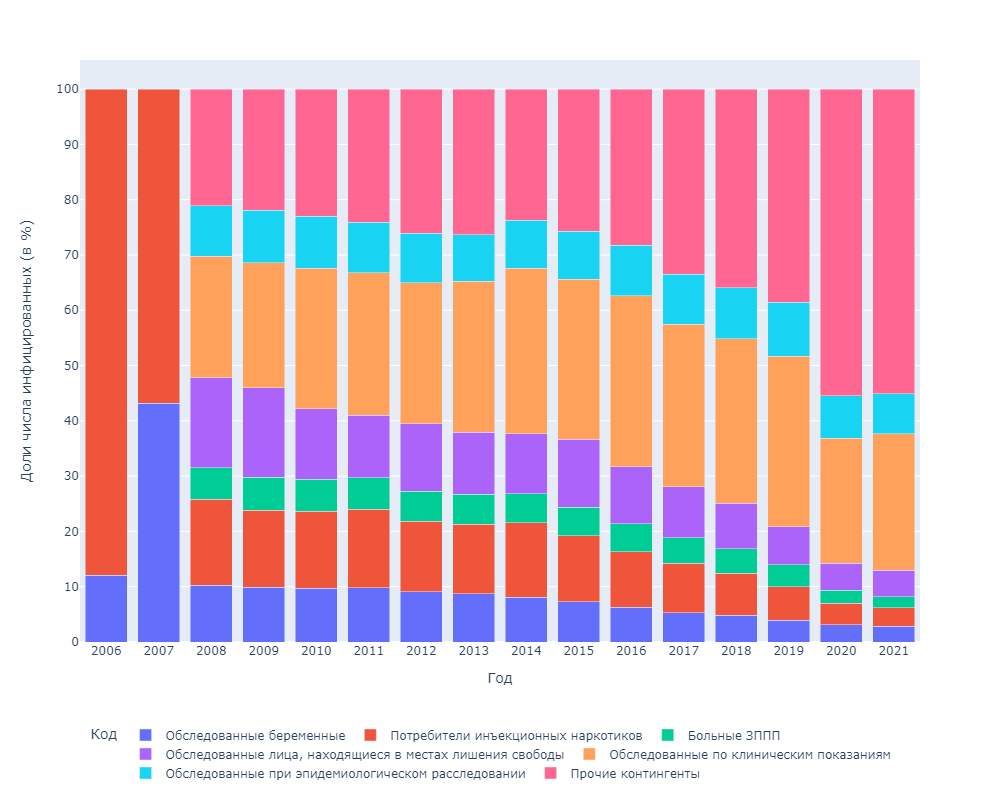
\includegraphics[width=1\textwidth]{f4_fractions}
	\caption{Распределение числа инфицированных по группам}
	\label{fig:f4_fractions}
\end{figure}

После прохождения процедур предобработки, все таблицы были соединены воедино, полученный результат и будет подаваться на вход модели машинного обучения. Всего в финальной таблице отражено 83 субъекта Российской Федерации, 34 социально-демографических предиктора и 2 целевые статистики: число новых случаев ВИЧ (НС), и уровень заболеваемости ВИЧ-инфекцией в просантимилле (НС \%).

Обратим внимание на то, что каждая из исходных таблиц содержала данные за разные промежутки времени, поэтому в результате их слияния было получено большое количество пропущенных значений. Проиллюстрируем количество колонок, имеющих в себе пропущенные значения, на рисунке \ref{fig:f4_missing}.
\newpage
\begin{figure}[ht]
	\centering
	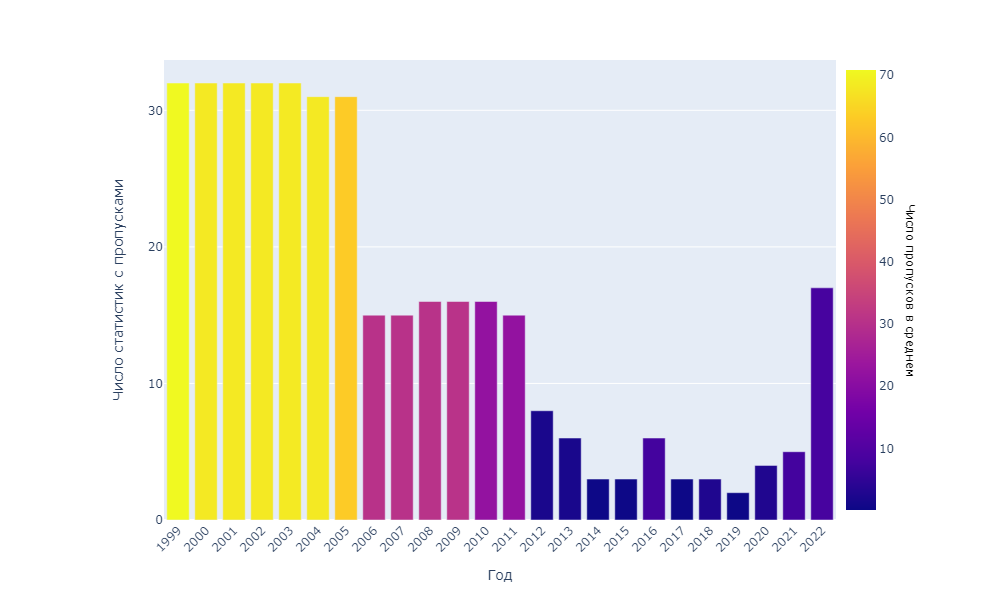
\includegraphics[width=1\textwidth]{missing_values_plot}
	\caption{Количество отсутствующих предикторов по годам}
	\label{fig:f4_missing}
\end{figure}


Как видно из графика, до 2005го года включительно большинство социально-демографических предикторов имеет очень большое количество пропусков. Начиная с 2006го года ситуация значительно улучшается, колонок с пропусками становится меньше, и в среднем число пропусков в каждой из них уменьшается вдвое. Кроме того, в 2022ом году статистика о заболеваемости ВИЧ-инфекцией на момент рассмотрения доступна лишь по малой части из субъектов. Учитывая эти факты, все наличные временные ряды будут рассмотрены в промежутке от 2006го до 2021 года включительно.

Для заполнения оставшихся пропусков были апробированы несколько методов:
\begin{itemize}
	\item заполнение предыдущим значением временного ряда;
	\item заполнение следующим значением временного ряда;
	\item заполнение пропущенных признаков с помощью линейной регрессии относительно наличных признаков.

\end{itemize}
 
 Как показали дальнейшие испытания, в целом качество предсказания всех моделей было выше в случае использования линейной регрессии, которая была реализована с применением класса <<Iterative Imputer>> из библиотеки <<scikit-learn>>.
 
\section{Описание используемых методов предсказания}

Для решения поставленной задачи машинного обучения были выбраны две наиболее перспективные нейросетевые архитектуры:

\begin{itemize}
	
	\item архитектура MES-LSTM, представляющая из себя комбинацию двойного экспоненциального сглаживания и рекуррентной нейронной сети;
	
	\item классическая рекуррентная архитектура LSTM без использования экспоненциального сглаживания.
	
\end{itemize} 

Для оценки эффективности использования нейросетевых моделей в сравнение также были добавлены классические статистические методы предсказания:
 
\begin{itemize}

	\item метод предсказания многомерных временных рядов VARMAX;
	
	\item метод предсказания одномерных временных рядов ARIMA.

\end{itemize}    

Опишем подробнее архитектуру MES-LSTM, представленную в 2021 году \cite{MES_RNN}. Структурная схема модели из оригинальной работы приведена на рисунке \ref{fig:MES_LSTM}.

\begin{figure}[h!]
	\centering
	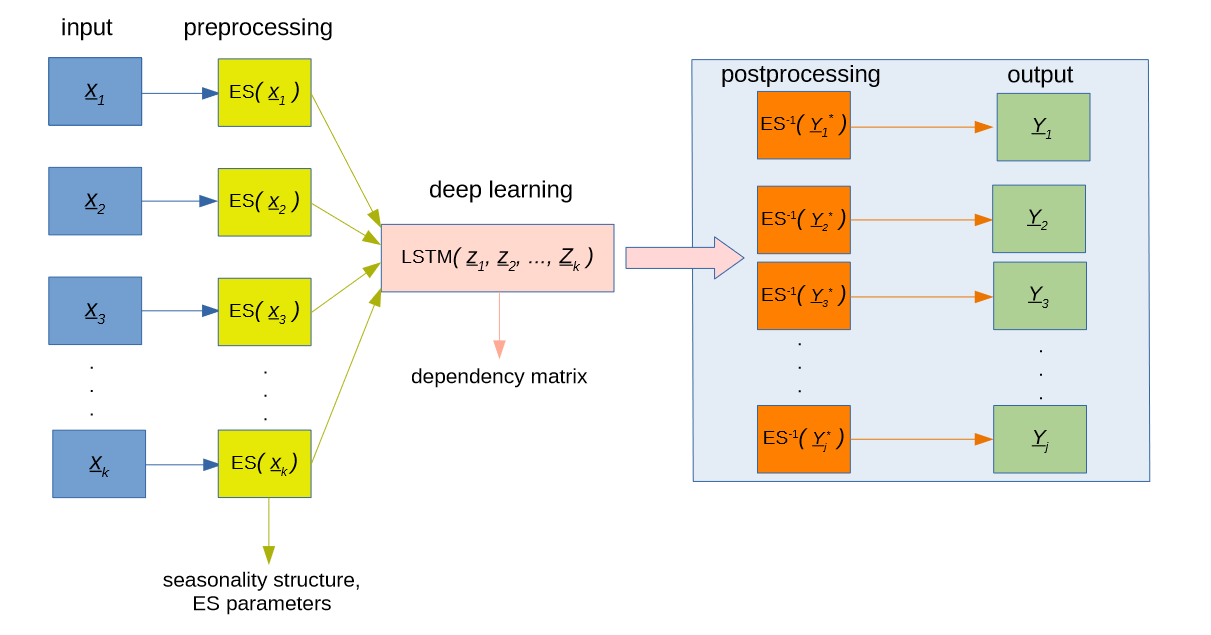
\includegraphics[width=0.9\textwidth]{MES_LSTM}
	\caption{Структурная схема модели MES-LSTM  \\
		Источник: [Mathonsi T., Zyl T.L. van. A Statistics and Deep Learning Hybrid Method for Multivariate Time Series Forecasting and Mortality Modeling  Forecasting. — 2022. — Mar. — Vol. 4, no. 11. — P. 1–25.]}
	\label{fig:MES_LSTM}
	
\end{figure}


\subsection{Слой предобработки (экспоненциальное сглаживание)}
Очищенные и масштабированные данные проходят через слой двойного экспоненциального сглаживания, где с помощью метода метода Хольта для каждой из временных последовательностей извлекается значения уровня и компоненты тренда. Пусть $y_t$ - фактическое значение временного ряда в момент времени $t$. Тогда каждое из значений $y_t$ может быть описано уравнением:

\begin{equation}
	\label{eq:LT_decompose}
	y_t=l_t + b_t + \epsilon_t,
\end{equation}
	

где $l_t$ - значение уровня в момент времени $t$;

 $b_t$ - значение тренда в момент времени $t$;
 
 $\epsilon_t$ - случайный шум с нулевым средним значением и постоянной дисперсией. 
 
Таким образом, в каждый момент времени текущее значение временного ряда складывается из некоторого базового значения (уровня), к которому прибавляется значение тренда (восходящего или нисходящего) и случайная величина ошибки.

Отметим, что в оригинальной работе и в задачах о прогнозировании временного ряда гораздо чаще используется тройное экспоненциальное сглаживание, позволяющее помимо тренда учитывать также сезонность (периодически повторяющиеся паттерны) в данных. Наши временные ряды, однако, представляются слишком короткими и имеют годичную периодичность, поэтому для сглаживания была выбрана упрощенная модель.

Для обучения алгоритма необходимо итеративно вычислить значения уровня и тренда для каждого момента времени, с помощью следующих уравнений:

\begin{equation}
	l_t = \alpha y_t + (1 - \alpha)(l_{t-1} + b_{t-1}),
\end{equation}

где $l_t$ - значения уровня в момент времени $t$;

	$\alpha$ - фактор сглаживания для уровня (0 ≤ $\alpha$ ≤ 1); 
	
	$y_t$ - фактическое значение временного ряда в момент времени $t$; 
	
	$l_{t-1}$ - значение уровня в предыдущий момент времени $t-1$;
	
	$b_{t-1}$ - значение тренда в предыдущий момент времени $t-1$.


 Коэффициент $\alpha$  определяет вес, придаваемый текущей точке данных ($y_t$) по сравнению с предыдущим сглаженным уровнем ($l_{t−1}$) и трендом ($b_{t-1}$). Более высокое значение $\alpha$ приводит к более быстрой реакции на изменения в фактических данных, то есть менее плавному сглаживанию.

\begin{equation}
	b_t = \gamma (l_t - l_{t-1}) + (1 - \gamma) b_{t-1},
\end{equation}
	
где $b_t$ - значение тренда в момент времени $t$; 

$\gamma$ - фактор сглаживания для тренда (0 ≤ $\gamma$ ≤ 1);

$l_t$ - значение уровня в момент времени $t$;

$l_{t-1}$  - значение уровня в предыдущий момент времени $t-1$;

$b_{t-1}$ - значение тренда в предыдущий момент времени $t-1$.

 
 Коэффициент $\gamma$ определяет вес, придаваемый изменению сглаженного уровня ($l_t - l_{t-1}$) по сравнению с предыдущим значением тренда ($b_{t-1}$). Более высокое значение коэффициента приводит к более быстрой реакции на изменение уровня, и, как следствие, более резкой смене тренда.
 
 
Начальные значения параметров инициализируются в модели следующим образом:

\begin{itemize}
	\item начальное значение уровня ($l_1$) приравнивается к первой точке во временной серии ($y_1$);
	
	\item начальный тренд равен нулю.
	
\end{itemize}

В процессе обучения коэффициенты $\alpha, \gamma$, а также начальные значения уровней $l_1, b_1$ выбираются наиболее оптимальным образом с помощью метода максимального правдоподобия. Когда процесс обучения завершен, для получения прогноза необходимо воспользоваться соотношением:

\begin{equation}
	\label{eq:forecasting_Holt}
	\hat{y}_{t+1} = l_t + b_t, 
\end{equation}

​где ​$\hat{y}_{t+1}$ - предсказанное значение ряда для следующего момента времени;

$l_t$ - значение уровня в момент времени $t$;

$b_t$ - значение тренда в момент времени $t$. 

Таким образом, прогноз на следующий период времени ($t+1$) - это сумма значений текущего уровня и текущего тренда.

В нашей модели, однако, экспоненциальное сглаживание не используется напрямую для получения предсказания в следующие моменты времени. Вместо этого, при помощи формулы (\ref{eq:LT_decompose}), из временного ряда извлекаются значения тренда каждой временной последовательности, на основе которых нейросеть LSTM архитектуры строит предсказания. 

Преобразованные временные ряды вместе формируют общую матрицу признаков $X$. Для получения предсказания используется не вся матрица признаков, а только несколько наиболее актуальных значений (так называемое окно обучения). Итоговое уравнение для получения предсказания нашей модели выглядит следующим образом:

\begin{equation}
	\label{eq:forecasting_MESRNN}
	\hat{y}_{t+1} = l_t + RNN(X_{t-size:t, k}),
\end{equation}


где $\hat{y}_{t+1}$ - предсказанное значение;

$l_t$ - значение уровня в момент $t$;

$RNN(X_{t-size:t, k})$ - предсказанное нейросетью значение тренда для момента времени $t$;

$X_{t-size:t, k}$ - срез наиболее актуальных значений матрицы $X$;

$size$ - размер окна обучения;

$k$ - количество предикторов.


\subsection{LSTM слой}

Матрица $X$, полученная на предыдущем шаге и содержащая значения трендов для каждой из временных последовательностей, итеративно, последовательностями по 3 наблюдения ($X_{t-size:t, k}$), подается на вход рекуррентной нейронной сети. Результатом работы модели является предсказанное значения тренда для уровня заболеваемости ВИЧ на текущий год ($\hat{b}_{t}$). 

Нейронная сеть включает в себя три слоя:
\begin{itemize}
	\item входной слой размерности (1, 3, $k$), где $k$ - количество предикторов в модели;
	\item скрытый LSTM слой, состоящий из 50ти нейронов;
	\item выходной слой типа DenseFlipout, позволяющий в процессе обучения получать оптимальное распределение весов для оценки границ доверительного интервала прогнозирования.
\end{itemize}

Структурное описание архитектуры нейросети, использованной для моделей LSTM и MES-LSTM, приведено в таблице \ref{tab:NN_Summary}. 

\begin{table}[ht]
	\caption{Структурная схема нейросети  }
	\label{tab:NN_Summary}
	\resizebox{\textwidth}{!}{%
		\begin{tabular}{lll}
			\hline
			Layer (type)                  & Output Shape                & Param \#                  \\ \hline
			lstm (LSTM)                   & \multicolumn{1}{c}{(1, 50)} & \multicolumn{1}{c}{17000} \\ \hline
			dense\_flipout (DenseFlipout) & \multicolumn{1}{c}{(1,2)}   & \multicolumn{1}{c}{202}   \\ \hline
			Total params: 17, 202         &                             &                           \\
			Trainable params: 17, 202     &                             &                           \\ \hline
			Non-trainable params: 0       &                             &                          
		\end{tabular}%
	}
\end{table}


\subsection{Процедура, обратная к сглаживанию}

Предсказанные на предыдущем этапе значения тренда заболеваемости ВИЧ складываются с извлеченными при сглаживании значениями уровня, в результате чего при помощи формулы (\ref{eq:forecasting_MESRNN}) получается предсказание на следующий момент времени. Таким образом, вместо использования значений локального линейного тренда $b_t$, который фигурирует в формуле для двойного экспоненциального сглаживания (\ref{eq:forecasting_Holt}), мы используем сложные значения нелинейного тренда, предсказанные нейросетью, которые призваны точнее описывать тенденции изучаемого временного ряда.

\section{Метрики оценки качества предсказания}

Для оценки качества предсказания были выбраны метрики MAPE и RMSE, определяемые с помощью формул:

\begin{equation}
	\text{MAPE} = \frac{100}{n} \sum_{t=1}^n \frac{\left|\hat{y}_t-y_t\right|}{y_t},
\end{equation}

где $n$ - количество значений в сравниваемых множествах;

$\hat{y}_t$ - предсказанное значение временного ряда;

$y_t$ - фактическое значение временного ряда.


\begin{equation}
	\text{RMSE} = \sqrt{\frac{1}{n} \sum_{i=1}^{n} (y_i - \hat{y}_i)^2},
\end{equation}

где $n$ - количество значений в сравниваемых множествах;

$y_t$ - фактическое значение временного ряда;

$\hat{y}_t$ - предсказанное значение временного ряда.

Метрика MAPE отражает среднюю процентную ошибку предсказания, метрика RMSE отражает среднеквадратичное отклонение предсказанных величин от фактических. Поскольку число новых случаев ВИЧ-инфекции в субъектах Российской Федерации колеблется от нескольких десятков до нескольких тысяч, обе метрики необходимы и вместе позволяют составить представление о точности работы каждой из моделей.

Как было упомянуто ранее, выбранные модели машинного обучения используются также и для оценки доверительного интервала предсказываемых значений. Это значит, что помимо непосредственно предсказанного значения временного ряда, в результате работы моделей мы получаем ещё пару значений, соответствующих нижней и верхней границе доверительного интервала. Для оценки точности предсказания границ доверительного интервала была использована метрика CS (coverage score), определяемая как:

\begin{equation}
	\text{CS} = \frac{1}{n} \sum_{i=1}^{n} [y_i \in CI_i],
\end{equation}

 где $n$ - количество предсказанных доверительных интервалов;
 
 $[ ]$ - нотация Айверсона;
 
 $y_i$ - фактическое значение временного ряда;
 
 $CI_i$ - предсказанный доверительный интервал для значения $y_i$.
 
 Метрика CS отображает долю фактических значений временного ряда, попавших в построенный для них доверительный интервал, что позволяет судить о точности построения доверительных интервалов.


\section{Поэтапное описание процесса получение предсказания}

Опишем целиком последовательность трансформаций, которую проходят исходные данные для извлечения из них предсказания:

\begin{enumerate}
	\item Производится подсчет количества пропусков в каждой из колонок исходной таблицы. Если процентное содержание пропусков слишком велико (больше 60 \%), колонка удаляется из таблицы.
	
	\item Все оставшиеся пропуски заполняются с помощью алгоритма <<Iterative Imputer>>, который использует линейную регрессию для восстановления пропущенных значений.
	
	\item Все признаки проходят процедуру масштабирования и центрирования таким образом, чтобы все численные значения таблицы находились в диапазоне (0,1). Такая процедура крайне рекомендована для любой модели машинного обучения, так как общем случае она позволяет алгоритму обучаться быстрее и точнее. В нашей работе для этого был использован метод, описанный в статье \cite{Умная_нормализация_данных_2020}.
	
	\item Предобработанные данные поступают в выбранные алгоритмы прогнозирования временных рядов, проходит обучение и получение предсказания на тестовых данных для каждой из моделей.
	
	\item С помощью выбранных метрик вычисляется невязка между полученными предсказаниями и реальными значениями тестовых данных.
	
	\item Полученные оценки используются для выбора наиболее точной модели, которая и будет использована для получения финального предсказания.

\end{enumerate}

\section{Сравнительный анализ качества используемых моделей}

Каждый из наличных временных рядов разбит на обучающую и тестовую части, до 2018 года и после 2019 года включительно. После завершения обучения каждый из выбранных методов был оценен по всем метрикам на тестовом множестве, для каждого субъекта Российской Федерации. Усредненные полученные оценки были использованы для выбора наилучшей модели.

Для валидации адекватности работы моделей были выбраны три субъекта Российской Федерации, значительно разнящиеся по количеству новых случаев заболевания за год и по форме временного ряда, а именно: 

\begin{itemize}
	\item Чукотский автономный округ (от 0 до 35 новых случаев заболевания);
	\item Свердловская область  (от 136 до 9337 новых случаев заболевания); 
	\item Томская область (от 0 до 1962 новых случаев заболевания).
\end{itemize}

Визуализируем историю обучения нейросети архитектуры MES-LSTM для каждой из выбранных областей.

\begin{figure}[ht!]
	\centering
	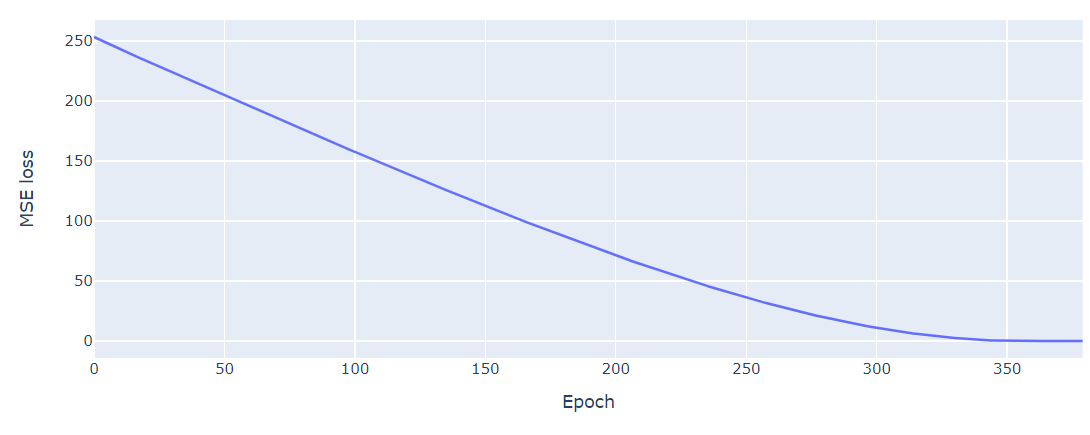
\includegraphics[width=0.8\textwidth]{images/chukotka_train_loss.png}
	\caption{MSE-loss в процессе обучения для Чуктоского АО}
	\label{fig:chukotka_train_score}
\end{figure}

\begin{figure}[h!]
	\centering
	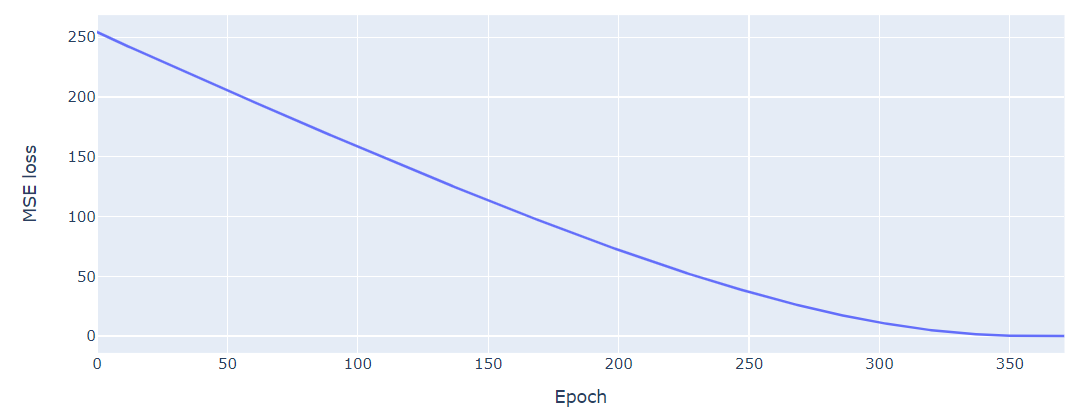
\includegraphics[width=0.8\textwidth]{images/sverdlovsk_train_loss}
	\caption{MSE-loss в процессе обучения для Свердловской области}
	\label{fig:sverdlovk_train_score}
\end{figure}

\begin{figure}[h!]
	\centering
	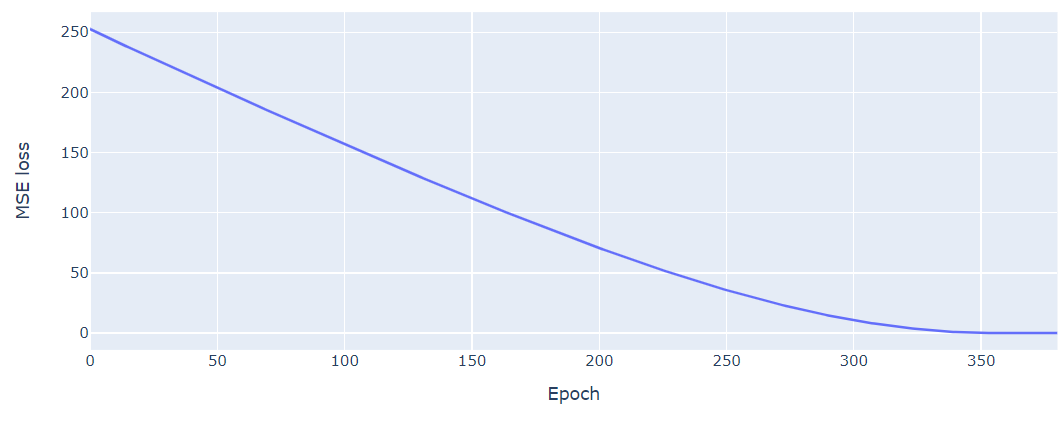
\includegraphics[width=0.8\textwidth]{images/tomsk_train_loss.png}
	\caption{MSE-loss в процессе обучения для Томской области}
	\label{fig:tomsk_train_score}
\end{figure}

Как видно из рисунков \ref{fig:chukotka_train_score}, \ref{fig:sverdlovk_train_score}, \ref{fig:tomsk_train_score}, в процессе обучения нейросеть смогла успешно минимизировать MSE-loss для всех трех областей, для этого потребовалось порядка 350 эпох.

Проиллюстрируем также предсказания, полученные с помощью всех методов, для каждой из выбранных областей.


\begin{figure}[ht]
	\centering
	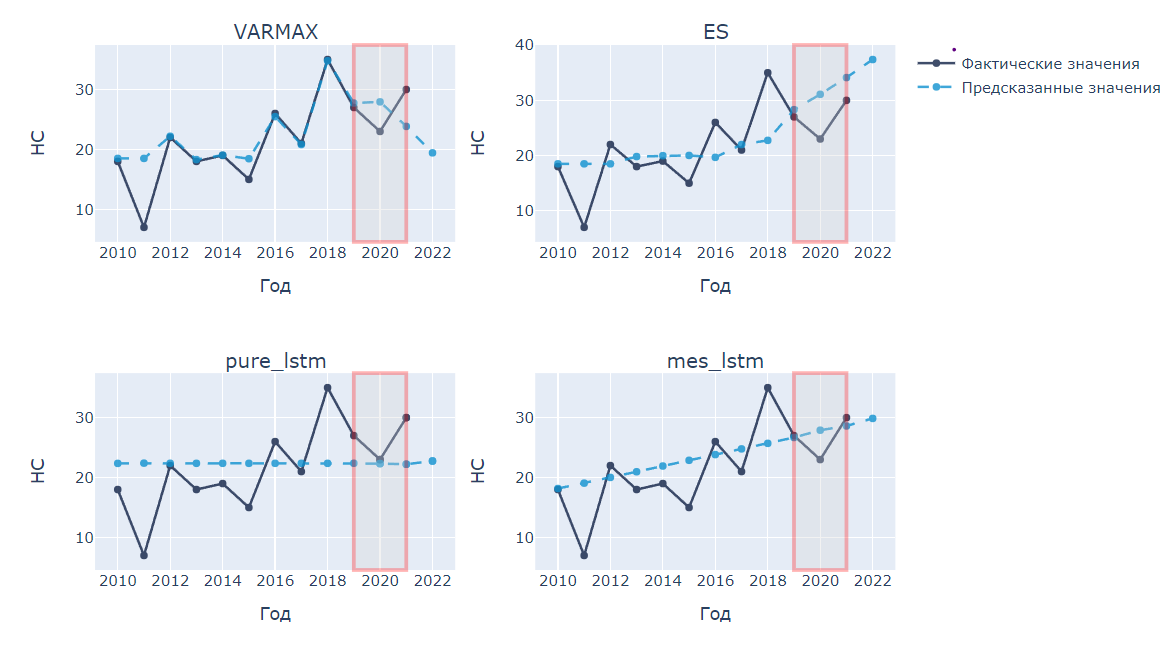
\includegraphics[width=1\textwidth]{images/chukotka_predict.png}
	\caption{Полученные предсказания для Чукотского АО}
	\label{fig:chukotka_predict}
\end{figure}

\begin{figure}[ht]
	\centering
	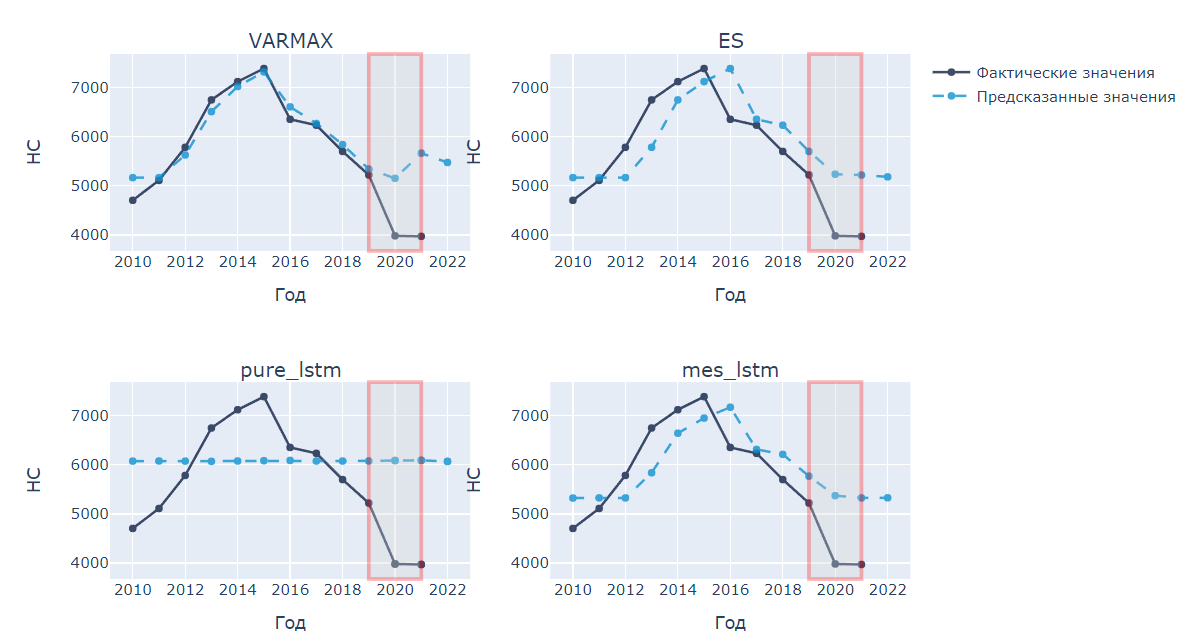
\includegraphics[width=1\textwidth]{images/sverdlovsk_predict.png}
	\caption{Полученные предсказания для Свердловской области}
	\label{fig:sverdlovsk_predict}
\end{figure}

\begin{figure}[ht]
	\centering
	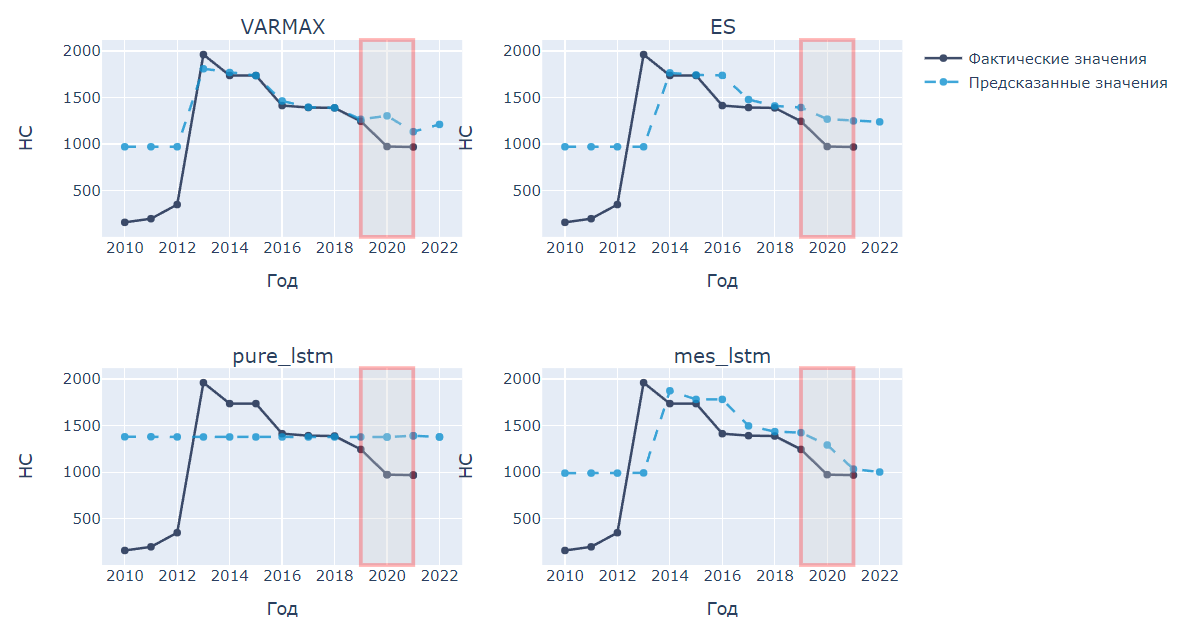
\includegraphics[width=1\textwidth]{images/tomsk_predict.png}
	\caption{Полученные предсказания для Томской области}
	\label{fig:tomsk_predict}
\end{figure}

Как видно из рисунков \ref{fig:chukotka_predict}, \ref{fig:sverdlovsk_predict}, \ref{fig:tomsk_predict}, все модели, кроме LSTM-нейросети в чистом виде, следуют за локальными трендами и строят разумные предсказания. LSTM в чистом виде, по всей видимости, не обучается должным образом, предсказывая каждый раз среднее значение по всему временному ряду. 

Приведем полученные на тестовом множестве и усредненные по субъектам Российской Федерации значения метрик для каждой из обученных моделей на рисунках \ref{fig:covmetric}, \ref{fig:mapemetric}, \ref{fig:rmsemetric}.

\begin{figure}[th]
	\centering
	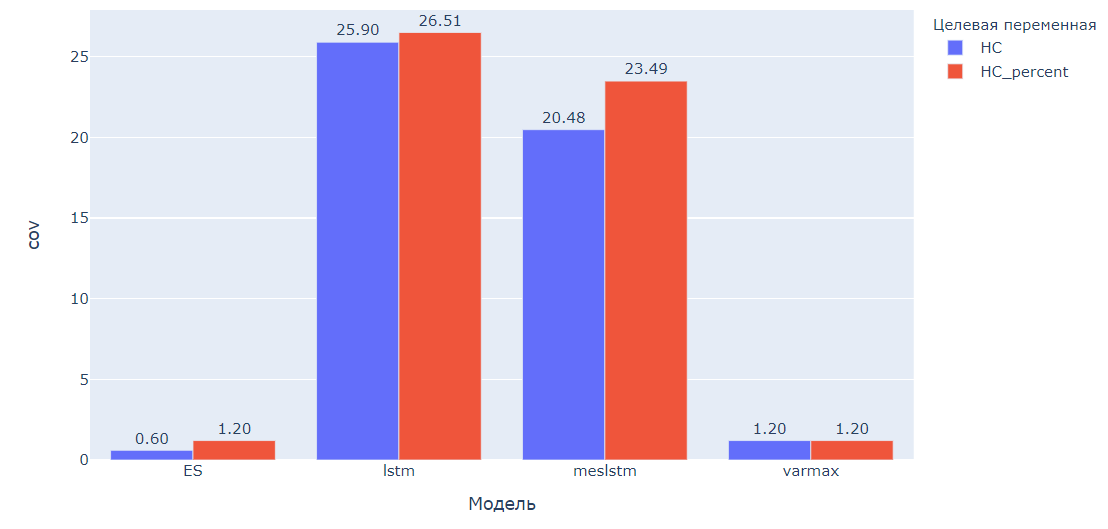
\includegraphics[width=1\textwidth]{images/cov_metric}
	\caption{Усредненное значение метрики COV для всех субъектов по каждой из моделей}
	\label{fig:covmetric}
\end{figure}

\begin{figure}[th]
	\centering
	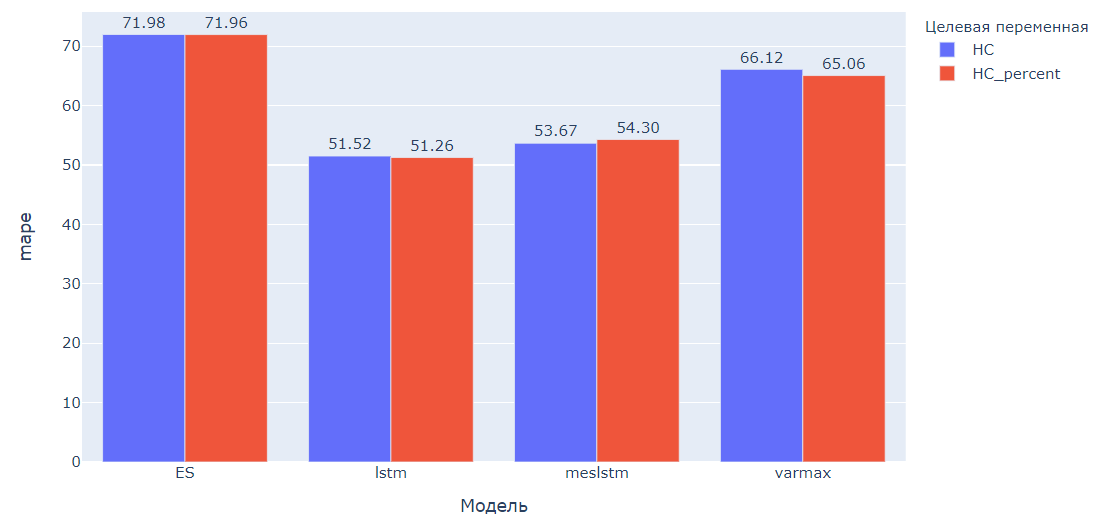
\includegraphics[width=1\textwidth]{images/mape_metric.png}
	\caption{Усредненное значение метрики MAPE для всех субъектов по каждой из моделей}
	\label{fig:mapemetric}
\end{figure}

\begin{figure}[th]
	\centering
	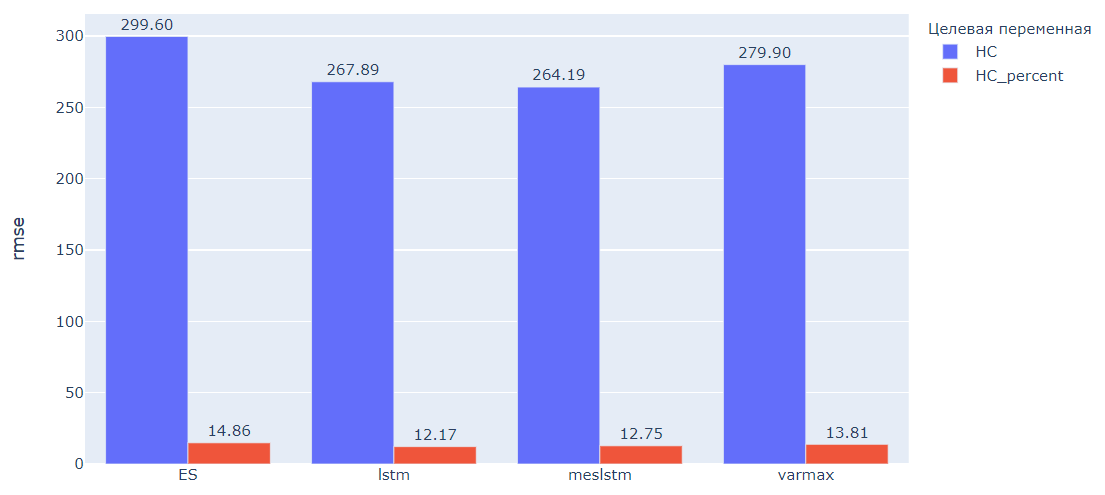
\includegraphics[width=1\textwidth]{images/rmse_metri}
	\caption{Усредненное значение метрики RMSE для всех субъектов по каждой из моделей}
	\label{fig:rmsemetric}
\end{figure}

Судя по приведенным значениям метрик, самой точной моделью оказалась нейросеть LSTM без использования экспоненциального сглаживания, сравнимый результат показала гибридная модель MES-LSTM. Модели VARMAX и ES показали худшее качество на всех метриках.

Таким образом, применение рекуррентной нейросети с использованием дополнительных социально-демографических факторов в нашей задаче позволило превзойти результаты классических статистических моделей. При этом, несмотря на формальное превосходство обыкновенной LSTM, для финального прогноза была выбрана гибридная модель MES-LSTM, как показавшая более разумный подход к предсказанию заболеваемости по результатам предсказаний для Свердловской и Томской областей, Чукотского автономного округа. 

\section{Полученный прогноз}

Модель, показавшая наибольшую точность, была использована для предсказания заболеваемости на 2022 год, с использованием наиболее актуальных данных. Полученные результаты приведены в  таблице \ref{tab:best_prediction}.

% Please add the following required packages to your document preamble:
% \usepackage{graphicx}
% \usepackage{lscape}
\begin{landscape}
	\begin{table}[]
		\caption{Предсказание лучшей модели на 2022 год}
		\label{tab:best_prediction}
		\resizebox{1.5\textwidth}{!} &
				\textbf{Территория} &
				\textbf{НС} &
				\textbf{HC\%} &
				\textbf{Территория} &
				\textbf{НС} &
				\textbf{HC\%} \\ \hline
				г. Санкт-Петербург                & 2510.0 & 48.10  & Ямало-Ненецкий АО               & 198.0  & 35.98  & Оренбургская область         & 1905.0 & 98.98  \\
				Республика Саха (Якутия)          & 165.0  & 16.80  & Московская область              & 3522.0 & 45.35  & Смоленская область           & 320.0  & 33.24  \\
				Чукотский АО                      & 30.0   & 59.12  & Брянская область                & 297.0  & 25.42  & Чеченская Республика         & 151.0  & 12.30  \\
				Республика Северная Осетия-Алания & 194.0  & 27.75  & Республика Татарстан            & 1117.0 & 28.78  & Ивановская область           & 540.0  & 52.94  \\
				Тульская область                  & 634.0  & 41.01  & Владимирская область            & 630.0  & 47.57  & Ленинградская область        & 1403.0 & 77.10  \\
				Новгородская область              & 393.0  & 64.50  & Астраханская область            & 220.0  & 22.43  & Республика Ингушетия         & 60.0   & 10.98  \\
				Липецкая область                  & 292.0  & 26.70  & Саратовская область             & 1134.0 & 46.19  & Омская область               & 1270.0 & 67.71  \\
				Сахалинская область               & 191.0  & 39.21  & Белгородская область            & 225.0  & 14.68  & Республика Калмыкия          & 24.0   & 8.75   \\
				Республика Коми                   & 445.0  & 55.96  & Республика Тыва                 & 48.0   & 14.56  & Еврейская автономная область & 51.0   & 32.70  \\
				Вологодская область               & 359.0  & 31.56  & Нижегородская область           & 1842.0 & 59.17  & Республика Карелия           & 260.0  & 34.11  \\
				Волгоградская область             & 821.0  & 31.59  & Карачаево-Черкесская Республика & 75.0   & 16.26  & Удмуртская Республика        & 1026.0 & 68.73  \\
				Свердловская область              & 5328.0 & 123.68 & Республика Адыгея               & 114.0  & 23.90  & Забайкальский край           & 432.0  & 42.63  \\
				Чувашская Республика              & 338.0  & 27.57  & Тамбовская область              & 223.0  & 21.83  & Иркутская область            & 2752.0 & 113.83 \\
				Республика Марий Эл               & 253.0  & 37.88  & Кемеровская область             & 4566.0 & 167.91 & Челябинская область          & 2978.0 & 86.44  \\
				г. Москва                         & 6843.0 & 54.21  & Курганская область              & 692.0  & 79.42  & Ставропольский край          & 661.0  & 23.04  \\
				Магаданская область               & 49.0   & 35.87  & Орловская область               & 209.0  & 29.22  & Калининградская область      & 451.0  & 44.89  \\
				Республика Мордовия               & 125.0  & 16.19  & Республика Алтай                & 89.0   & 39.96  & Томская область              & 1002.0 & 93.61  \\
				Новосибирская область             & 2854.0 & 106.82 & Камчатский край                 & 149.0  & 48.04  & Калужская область            & 344.0  & 34.18  \\
				Воронежская область               & 635.0  & 27.55  & Ханты-Мансийский АО-Югра        & 1203.0 & 78.67  & Республика Башкортостан      & 2260.0 & 55.93  \\
				Ярославская область               & 524.0  & 41.43  & Псковская область               & 158.0  & 25.76  & Курская область              & 242.0  & 22.42  \\
				Ростовская область                & 1630.0 & 38.74  & Пермский край                   & 2559.0 & 95.40  & Республика Бурятия           & 588.0  & 59.89  \\
				Мурманская область                & 394.0  & 51.61  & Тверская область                & 724.0  & 57.63  & Республика Дагестан          & 419.0  & 12.63  \\
				Архангельская область без АО &
				321.0 &
				30.10 &
				Красноярский край &
				2730.0 &
				95.69 &
				Кабардино-Балкарская Республика &
				250.0 &
				28.80 \\
				Амурская область                  & 212.0  & 27.30  & Краснодарский край              & 2343.0 & 40.83  &                              &        &        \\
				Самарская область                 & 3492.0 & 109.01 & Пензенская область              & 405.0  & 31.87  &                              &        &        \\
				Ненецкий АО                       & 12.0   & 26.47  & Ульяновская область             & 902.0  & 70.91  &                              &        &        \\
				Алтайский край                    & 2182.0 & 100.54 & Кировская область               & 153.0  & 12.14  &                              &        &        \\
				Рязанская область                 & 252.0  & 23.17  & Приморский край                 & 959.0  & 51.14  &                              &        &        \\
				Тюменская область без АО          & 1174.0 & 90.25  & Хабаровский край                & 375.0  & 28.83  &                              &        &        \\
				Республика Хакасия                & 317.0  & 60.09  & Костромская область             & 240.0  & 38.76  &                              &        &        \\ \hline
			\end{tabular}%
		}
	\end{table}
\end{landscape}



\endinput                                  % Третья глава
\chapter*{Заключение}
\label{ch:conclusion}
\linespread{1.5}
В рамках выпускной квалификационной работы выполнены следующие задачи:

\begin{enumerate}
	\item Cобрана и изучена статистика заболеваемости ВИЧ-инфекцией в субъектах Российской Федерации, сформулирована актуальность и важность рассматриваемой проблемы.
	
	\item Произведен литературный анализ работ, посвященных социально-демографическим факторам, способствующим распространению ВИЧ-инфекции в России и в зарубежных странах, по наиболее важным факторам собрана и изучена статистика.  
	
	\item Все собранные статистики очищены от пропусков, дубликатов, аномальных значений, наименования субъектов приведены к единому стандарту, все данные агрегированы в едином носителе (таблице).
	
	\item Проведен литературный анализ работ посвященных методам прогнозирования эпидемиологических процессов, включая статистические методы и методы машинного обучения. Наиболее перспективные методы добавлены в сравнение.
	
	\item Для оценки качества прогностических моделей выбраны метрики, разработана стратегия машинного обучения.
	
	\item Выбранные модели реализованы программно, проведены эксперименты по обучению моделей и получению прогнозов, результаты представлены графически.
	
	\item В соответствии с результатами проведена работа по оптимизации параметров каждой из моделей, с использованием подобранных параметров получен финальный прогноз заболеваемости для каждого из субъектов Российской Федерации.
	
\end{enumerate}

Полученные в ходе выпускной квалификационной работы результаты позволяют судить о применимости и эффективности новейших методов машинного обучения в задачах о прогнозировании эпидемиологических процессов, извлеченные знания позволят в дальнейшем строить и оптимизировать более точные, совершенные модели.

Практическим результатом проведенной работы является прогноз заболеваемости ВИЧ-инфекции с использованием наиболее актуальных данных. С получением новых данных полученная модель может быть дообучена и использована повторно для предсказания заболеваемости ВИЧ-инфекции в последующих годах. Полученная информация далее может быть проанализирована и использована органами здравоохранения для более эффективного распределения ресурсов и проведения профилактических мероприятий в субъектах Российской Федерации. 


\endinput                                  % Третья глава

\printbibliography[title=Список использованных источников] % Автособираемый список литературы

\end{document}
